% Author: Aurelia Wang
% Editor: Dun-Ming Huang, on formatting
% Author Email: aureliawang@berkeley.edu
% CSM16A Spring 2023

\qns{State Transition Inverses}\\
\editnotes{
    I restructured the answers and some paragraph breaks to make file slightly more readable for SM reviewers. \\
    I did not change any bold/italicize contents in, so to preserve original intentions of content.

}

\meta{
\begin{itemize}
    \item Remind students how to create a transition matrix from analyzing a state transition diagram
    
    \item Explain to students why taking the inverse of the transition matrix is what happens at the previous timestep. Show how $\vec{x}[t]=\textbf{T}\vec{x}[t-1]$, so therefore 
    ${T^{-1}}\vec{x}[t]=\vec{x}[t-1]$.

    \item Go over the steps of taking an inverse of a matrix
\end{itemize}
}

STEM students in Berkeley regularly move across three engineering buildings: Soda, Cory, and Sutardja Dai. 
\begin{enumerate}
\item {You want to analyze the dynamics of foot traffic and end up constructing this transition diagram:

% Author: Aurelia Wang
% Email: aureliawang@berkeley.edu
% CSM16A Spring 2023

\begin{center}
    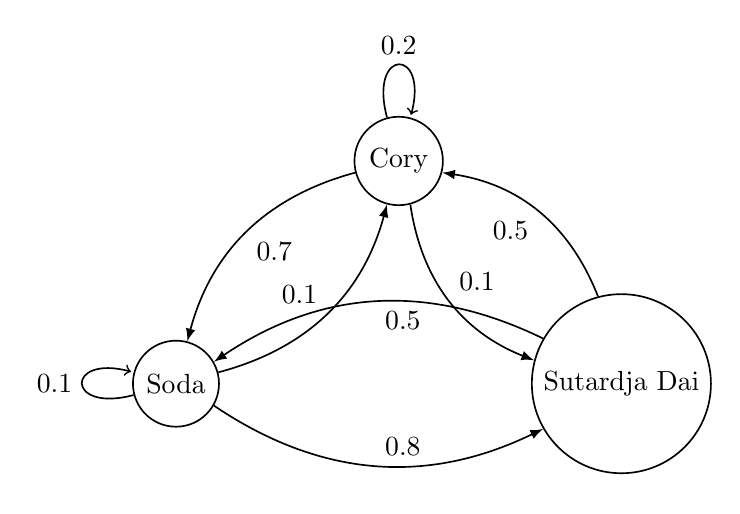
\begin{tikzpicture}[-latex, auto, node distance={4cm}, semithick, main/.style = {draw, circle}]
        \node[main] (Cory) {Cory};
        \node[main, below left of = Cory] (Soda) {Soda};
        \node[main, below right of = Cory] (Sutardja Dai) {Sutardja Dai};
        \path (Cory) edge[loop above] node{0.2} (Cory);
        \path (Cory) edge[bend right] node{0.7} (Soda);
        \path (Cory) edge[bend right] node{0.1} (Sutardja Dai);
        \path (Soda) edge[bend right] node{0.1} (Cory);
        \path (Soda) edge[loop left] node{0.1} (Soda);
        \path (Soda) edge[bend right] node{0.8} (Sutardja Dai);
        \path (Sutardja Dai) edge[bend right] node{0.5} (Cory);
        \path (Sutardja Dai) edge[bend right] node{0.5} (Soda);
    \end{tikzpicture}
\end{center}

The current number of students at each time-step \emph{t} is given by the state vector $\vec{x}[t]$ defined as:
\begin{align}
    \vec{x}[t] &= \begin{bmatrix}
           x_{So}[t] \\
           x_{Co}[t] \\
           x_{Su}[t]
         \end{bmatrix}
  \end{align}

where $x_{So}[t]$ denotes the number of students in Soda at time \emph{t}, $x_{Co}[t]$ denotes the number of students in Cory at time \emph{t}, and $x_{Su}[t]$ denotes the number of students in Sutardja Dai at time \emph{t}.

\vspace{5mm} %5mm vertical space

Explicitly write out the transition matrix \textbf{T} from the provided diagram such that $\vec{x}[t + 1] = \textbf{T} \vec{x}[t]$. Is the system conservative? Justify your answer.

\begin{align}
    \textbf{T} &= \begin{bmatrix}
          & & & & & & \\
          & & & & & & \\
          & & & & & & \\
          & & & & & &
         \end{bmatrix}
  \end{align}

\vspace{5mm} %5mm vertical space
}
\ans{
    The correct transition matrix is 
    \begin{align}
    \textbf{T} &= \begin{bmatrix}
          0.2 & 0.1 & 0.5 \\
          0.7 & 0.1 & 0.5 \\
          0.1 & 0.8 & 0 \\
         \end{bmatrix}
  \end{align}
  where the columns represent the location that students are moving from while the each row represents the location students are moving to in that timestep. Because each column sums up to 1, the system is conservative and no students are lost or gained inbetween each timestep. When you learn eigenvalues and eigenvectors, we will be able to better understand the steady state of transition matrices and how the overall system converges.
}
\item {If 
\begin{align}
    \vec{x}[t] &= \begin{bmatrix}
          100  \\
          50  \\
          50  \\
         \end{bmatrix}
  \end{align}
would it be possible to determine the state vector at the previous timestep \emph{t} - 1? 
}
% \begin{align}
%     \vec{x}[t-1] &= \begin{bmatrix}
%           & &  \\
%           & &  \\
%           & &  \\
%          \end{bmatrix}
%   \end{align}

\vspace{5mm} %5mm vertical space
\ans{
    By checking whether $T^{-1}$ exists through Gaussian Elimination, we end up with a matrix of 
  \begin{align}
    \textbf{T} &= \begin{bmatrix}
          1 & 0 & 0 \\
          0 & 1 & 0 \\
          0 & 0 & 1 \\
         \end{bmatrix}
  \end{align}
  Because there are unique pivot columns, \textbf{T} does have an inverse, and thus it would be possible to determine the previous state at timestep \emph{t} - 1.
  The inverse of this matrix is as follows (but calculating this is optional):
  \begin{align}
    T^{-1} &= \begin{bmatrix}
          -2 & -2 & 0 \\
          0.25 & -0.25 & 1.25 \\
          2.75 & -0.75 & -0.25 \\
         \end{bmatrix}
  \end{align}
}

\item {Is it possible to find the state of the transition matrix at timestep \emph{n-2}? You do not need to calculate this; just explain the conditions under which it would be possible and wouldn't be.}

\ans{
    It is possible to find the state of $\vec{x}[t-2]$ because $T^{-1}$ itself is invertible. The conditions in which it would be invertible if $T^{-1}$ is completely linearly independent, which can be found through Gaussian Elimination.
}

\vspace{5mm} %5mm vertical space

\item {Suppose you are given a new transition matrix:
\begin{align}
    \textbf{T} &= \begin{bmatrix}
          0 & 0.5 & 0.5 \\
          0.2 & 0.3 & 0.5 \\
          0.4 & 0.6 & 0 \\
         \end{bmatrix}
  \end{align}
  where the columns sum up to 1 but the rows do not. Does this new matrix tell us anything about the foot traffic?
}
\ans{
This system is not conservative because the columns do not add up to 1, so either there will be increasingly less students in the total system at each timestep, or there will be more. The columns summing to 1 does not have a real significance; just keep in mind that rows summing to one means the system is conservative, but not if the columns sum to 1.
}
\end{enumerate}
